\newpage
% % 11 round differential 
% %==============================================================================================
\renewcommand{\arraystretch}{1.5} % Adjust the row height
\setlength{\tabcolsep}{0pt} % Remove extra padding between columns

\caption{ 11 round differential}
\begin{center}
    \resizebox{\textwidth}{!}{%
        \(
        \begin{array}{|p{0.5cm}|p{0.5cm}|p{0.5cm}|p{0.5cm}|}
            \hline
            ?    & ?    & ?    & ?    \\ \hline
            \ast & ?    & ?    & \ast \\ \hline
            \ast & \ast & ?    & ?    \\ \hline
            \ast & ?    & \ast & ?    \\ \hline
        \end{array}
        \hspace{2pt} % Decrease space here
        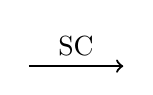
\begin{tikzpicture}[baseline={(current bounding box.center)}, scale=0.4]
            % Arrow from first grid to second grid
            \draw[->, thick] (0, 0) -- (3, 0)
            node[midway, above] {SC};
        \end{tikzpicture}
        \hspace{2pt} % Decrease space here
        \begin{array}{|p{0.5cm}|p{0.5cm}|p{0.5cm}|p{0.5cm}|}
            \hline
            ?    & ?    & ?    & ?    \\ \hline
            \ast & ?    & ?    & \ast \\ \hline
            \ast & \ast & ?    & ?    \\ \hline
            \ast & ?    & \ast & ?    \\ \hline
        \end{array}
        \hspace{2pt} % Decrease space here
        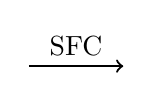
\begin{tikzpicture}[baseline={(current bounding box.center)}, scale=0.4]
            % Arrow from second grid to third grid
            \draw[->, thick] (0, 0) -- (3, 0)
            node[midway, above] {SFC};
        \end{tikzpicture}
        \hspace{2pt} % Decrease space here
        \begin{array}{|p{0.5cm}|p{0.5cm}|p{0.5cm}|p{0.5cm}|}
            \hline
            ? & ?    & ?    & ?    \\ \hline
            ? & ?    & \ast & \ast \\ \hline
            ? & \ast & ?    & \ast \\ \hline
            ? & \ast & \ast & ?    \\ \hline
        \end{array}
        \hspace{2pt} % Decrease space here
        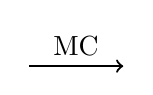
\begin{tikzpicture}[baseline={(current bounding box.center)}, scale=0.4]
            % Arrow from third grid to fourth grid
            \draw[->, thick] (0, 0) -- (3, 0)
            node[midway, above] {MC};
        \end{tikzpicture}
        \hspace{2pt} % Decrease space here
        \begin{array}{|p{0.5cm}|p{0.5cm}|p{0.5cm}|p{0.5cm}|}
            \hline
                 &      &      &      \\ \hline
            \ast &      & \ast & \ast \\ \hline
            \ast & \ast &      & \ast \\ \hline
            \ast & \ast & \ast &      \\ \hline
        \end{array}
        \)
        \hspace{2pt} % Decrease space here

        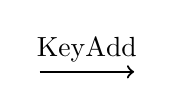
\begin{tikzpicture}[baseline={(current bounding box.center)}, scale=0.4]
            % Arrow from third grid to fourth grid
            \draw[->, thick] (0, 0) -- (3, 0)
            node[midway, above] {KeyAdd};
        \end{tikzpicture}

    }
\end{center}
\begin{center}
    \resizebox{\textwidth}{!}{%
        \(
        \begin{array}{|p{0.5cm}|p{0.5cm}|p{0.5cm}|p{0.5cm}|}
            \hline
                 &      &      &      \\ \hline
            \ast &      & \ast & \ast \\ \hline
            \ast & \ast &      & \ast \\ \hline
            \ast & \ast & \ast &      \\ \hline
        \end{array}
        \hspace{2pt} % Decrease space here
        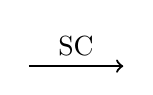
\begin{tikzpicture}[baseline={(current bounding box.center)}, scale=0.4]
            % Arrow from first grid to second grid
            \draw[->, thick] (0, 0) -- (3, 0)
            node[midway, above] {SC};
        \end{tikzpicture}
        \hspace{2pt} % Decrease space here
        \begin{array}{|p{0.5cm}|p{0.5cm}|p{0.5cm}|p{0.5cm}|}
            \hline
                     &          &          &          \\ \hline
            \Delta_1 &          & \Delta_2 & \Delta_3 \\ \hline
            \Delta_3 & \Delta_2 &          & \Delta_1 \\ \hline
            \Delta_2 & \Delta_3 & \Delta_1 &          \\ \hline
        \end{array}
        \hspace{2pt} % Decrease space here
        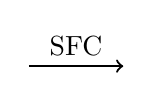
\begin{tikzpicture}[baseline={(current bounding box.center)}, scale=0.4]
            % Arrow from second grid to third grid
            \draw[->, thick] (0, 0) -- (3, 0)
            node[midway, above] {SFC};
        \end{tikzpicture}
        \hspace{2pt} % Decrease space here
        \begin{array}{|p{0.5cm}|p{0.5cm}|p{0.5cm}|p{0.5cm}|}
            \hline
             & \Delta_1 & \Delta_2 & \Delta_3 \\ \hline
             &          & \Delta_2 & \Delta_3 \\ \hline
             & \Delta_1 &          & \Delta_3 \\ \hline
             & \Delta_1 & \Delta_2 &          \\ \hline
        \end{array}
        \hspace{2pt} % Decrease space here
        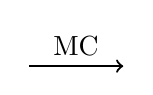
\begin{tikzpicture}[baseline={(current bounding box.center)}, scale=0.4]
            % Arrow from third grid to fourth grid
            \draw[->, thick] (0, 0) -- (3, 0)
            node[midway, above] {MC};
        \end{tikzpicture}
        \hspace{2pt} % Decrease space here
        \begin{array}{|p{0.5cm}|p{0.5cm}|p{0.5cm}|p{0.5cm}|}
            \hline
             &      &      &      \\ \hline
             & \ast &      &      \\ \hline
             &      & \ast &      \\ \hline
             &      &      & \ast \\ \hline
        \end{array}
        \)
        \hspace{2pt} % Decrease space here
        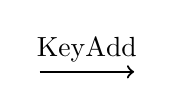
\begin{tikzpicture}[baseline={(current bounding box.center)}, scale=0.4]
            % Arrow from third grid to fourth grid
            \draw[->, thick] (0, 0) -- (3, 0)
            node[midway, above] {KeyAdd};
        \end{tikzpicture}

    }
\end{center}
\begin{center}
    \resizebox{\textwidth}{!}{%
        \(
        \begin{array}{|p{0.5cm}|p{0.5cm}|p{0.5cm}|p{0.5cm}|}
            \hline
             &      &      &      \\ \hline
             & \ast &      &      \\ \hline
             &      & \ast &      \\ \hline
             &      &      & \ast \\ \hline
        \end{array}
        \hspace{2pt} % Decrease space here
        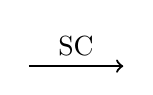
\begin{tikzpicture}[baseline={(current bounding box.center)}, scale=0.4]
            % Arrow from first grid to second grid
            \draw[->, thick] (0, 0) -- (3, 0)
            node[midway, above] {SC};
        \end{tikzpicture}
        \hspace{2pt} % Decrease space here
        \begin{array}{|p{0.5cm}|p{0.5cm}|p{0.5cm}|p{0.5cm}|}
            \hline
             &        &        &        \\ \hline
             & \delta &        &        \\ \hline
             &        & \delta &        \\ \hline
             &        &        & \delta \\ \hline
        \end{array}
        \hspace{2pt} % Decrease space here
        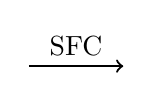
\begin{tikzpicture}[baseline={(current bounding box.center)}, scale=0.4]
            % Arrow from second grid to third grid
            \draw[->, thick] (0, 0) -- (3, 0)
            node[midway, above] {SFC};
        \end{tikzpicture}
        \hspace{2pt} % Decrease space here
        \begin{array}{|p{0.5cm}|p{0.5cm}|p{0.5cm}|p{0.5cm}|}
            \hline
                   &  &  & \\ \hline
            \delta &  &  & \\ \hline
            \delta &  &  & \\ \hline
            \delta &  &  & \\ \hline
        \end{array}
        \hspace{2pt} % Decrease space here
        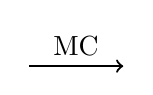
\begin{tikzpicture}[baseline={(current bounding box.center)}, scale=0.4]
            % Arrow from third grid to fourth grid
            \draw[->, thick] (0, 0) -- (3, 0)
            node[midway, above] {MC};
        \end{tikzpicture}
        \hspace{2pt} % Decrease space here
        \begin{array}{|p{0.5cm}|p{0.5cm}|p{0.5cm}|p{0.5cm}|}
            \hline
            \delta &  &  & \\ \hline
                   &  &  & \\ \hline
                   &  &  & \\ \hline
                   &  &  & \\ \hline
        \end{array}
        \)
        \hspace{2pt} % Decrease space here
        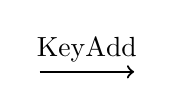
\begin{tikzpicture}[baseline={(current bounding box.center)}, scale=0.4]
            % Arrow from third grid to fourth grid
            \draw[->, thick] (0, 0) -- (3, 0)
            node[midway, above] {KeyAdd};
        \end{tikzpicture}

    }
\end{center}

%==============================================================begin================================
\(
\begin{array}{|p{0.5cm}|p{0.5cm}|p{0.5cm}|p{0.5cm}|}
    \hline
    \delta &  &  & \\ \hline
           &  &  & \\ \hline
           &  &  & \\ \hline
           &  &  & \\ \hline
\end{array}
\hspace{20pt}
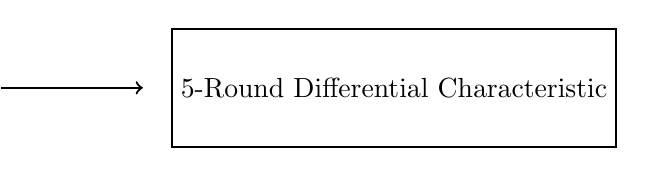
\begin{tikzpicture}[baseline={(current bounding box.center)}, scale=0.6]

    % Arrow to 5-round Differential Characteristic
    \node[draw, thick, minimum height=1.5cm, minimum width=4.5cm, anchor=west] (box) at (0, 0) {5-Round Differential Characteristic};
    \hspace{-10pt}
    \draw[->, thick] (-3, 0) -- (box.west);

    % Outputs: Y_0, Z_0, W_0
    % \node[right=0.5cm of box.east] (Y0) {$Y_0$};
    % \node[right=1.5cm of Y0] (Z0) {$Z_0$};
    % \node[right=1.5cm of Z0] (W0) {$W_0$};

    % Connecting arrows
    % \draw[->, thick] (box.east) -- (Y0.west);

\end{tikzpicture}
\)
% %==============================================================================================
\begin{center}
    \resizebox{\textwidth}{!}{%
        \(
        \begin{array}{|p{0.5cm}|p{0.5cm}|p{0.5cm}|p{0.5cm}|}
            \hline
            A &  & F &   \\ \hline
            A &  & F & 5 \\ \hline
              &  & 5 & 5 \\ \hline
              &  & A & 5 \\ \hline
        \end{array}
        \hspace{2pt} % Decrease space here
        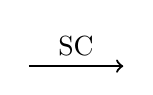
\begin{tikzpicture}[baseline={(current bounding box.center)}, scale=0.4]
            % Arrow from first grid to second grid
            \draw[->, thick] (0, 0) -- (3, 0)
            node[midway, above] {SC};
        \end{tikzpicture}
        \hspace{2pt} % Decrease space here
        \begin{array}{|p{0.5cm}|p{0.5cm}|p{0.5cm}|p{0.5cm}|}
            \hline
            \ast &        & \ast &      \\ \hline
            \ast & \delta & \ast &      \\ \hline
                 &        & \ast & \ast \\ \hline
                 &        & \ast & \ast \\ \hline
        \end{array}
        \hspace{2pt} % Decrease space here
        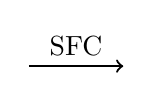
\begin{tikzpicture}[baseline={(current bounding box.center)}, scale=0.4]
            % Arrow from second grid to third grid
            \draw[->, thick] (0, 0) -- (3, 0)
            node[midway, above] {SFC};
        \end{tikzpicture}
        \hspace{2pt} % Decrease space here
        \begin{array}{|p{0.5cm}|p{0.5cm}|p{0.5cm}|p{0.5cm}|}
            \hline
            \ast & \ast & \ast &      \\ \hline
            \ast &      &      & \ast \\ \hline
                 & \ast & \ast &      \\ \hline
            \ast & \ast &      & \ast \\ \hline
        \end{array}
        \hspace{2pt} % Decrease space here
        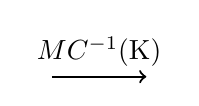
\begin{tikzpicture}[baseline={(current bounding box.center)}, scale=0.4]
            % Arrow from third grid to fourth grid
            \draw[->, thick] (0, 0) -- (3, 0)
            node[midway, above] {$MC^{-1}$(K)};
        \end{tikzpicture}
        \hspace{2pt} % Decrease space here
        \begin{array}{|p{0.5cm}|p{0.5cm}|p{0.5cm}|p{0.5cm}|}
            \hline
            \ast & \ast & \ast &      \\ \hline
            \ast &      &      & \ast \\ \hline
                 & \ast & \ast &      \\ \hline
            \ast & \ast &      & \ast \\ \hline
        \end{array}
        \)
        \hspace{2pt} % Decrease space here
        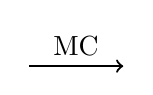
\begin{tikzpicture}[baseline={(current bounding box.center)}, scale=0.4]
            % Arrow from third grid to fourth grid
            \draw[->, thick] (0, 0) -- (3, 0)
            node[midway, above] {MC};
        \end{tikzpicture}

    }
\end{center}

\begin{center}
    \resizebox{\textwidth}{!}{%
        \(
        \begin{array}{|p{0.5cm}|p{0.5cm}|p{0.5cm}|p{0.5cm}|}
            \hline
            ? & ? &      & ?    \\ \hline
            ? & ? & \ast & \ast \\ \hline
            ? & ? & \ast & ?    \\ \hline
            ? & ? & \ast & \ast \\ \hline
        \end{array}
        \hspace{2pt} % Decrease space here
        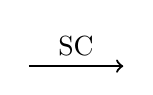
\begin{tikzpicture}[baseline={(current bounding box.center)}, scale=0.4]
            % Arrow from first grid to second grid
            \draw[->, thick] (0, 0) -- (3, 0)
            node[midway, above] {SC};
        \end{tikzpicture}
        \hspace{2pt} % Decrease space here
        \begin{array}{|p{0.5cm}|p{0.5cm}|p{0.5cm}|p{0.5cm}|}
            \hline
            ? & ? &      & ?    \\ \hline
            ? & ? & \ast & \ast \\ \hline
            ? & ? & \ast & ?    \\ \hline
            ? & ? & \ast & \ast \\ \hline
        \end{array}
        \hspace{2pt} % Decrease space here
        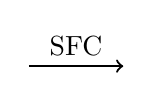
\begin{tikzpicture}[baseline={(current bounding box.center)}, scale=0.4]
            % Arrow from second grid to third grid
            \draw[->, thick] (0, 0) -- (3, 0)
            node[midway, above] {SFC};
        \end{tikzpicture}
        \hspace{2pt} % Decrease space here
        \begin{array}{|p{0.5cm}|p{0.5cm}|p{0.5cm}|p{0.5cm}|}
            \hline
            ?    & ?    & \ast & ?    \\ \hline
            \ast & ?    & ?    & \ast \\ \hline
            ?    & \ast & ?    & ?    \\ \hline
            \ast & ?    & ?    &      \\ \hline
        \end{array}
        \hspace{2pt} % Decrease space here
        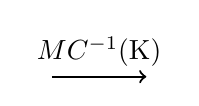
\begin{tikzpicture}[baseline={(current bounding box.center)}, scale=0.4]
            % Arrow from third grid to fourth grid
            \draw[->, thick] (0, 0) -- (3, 0)
            node[midway, above] {$MC^{-1}$(K)};
        \end{tikzpicture}
        \hspace{2pt} % Decrease space here
        \begin{array}{|p{0.5cm}|p{0.5cm}|p{0.5cm}|p{0.5cm}|}
            \hline
            ?    & ?    & \ast & ?    \\ \hline
            \ast & ?    & ?    & \ast \\ \hline
            ?    & \ast & ?    & ?    \\ \hline
            \ast & ?    & ?    &      \\ \hline
        \end{array}
        \)
        \hspace{2pt} % Decrease space here
        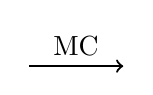
\begin{tikzpicture}[baseline={(current bounding box.center)}, scale=0.4]
            % Arrow from third grid to fourth grid
            \draw[->, thick] (0, 0) -- (3, 0)
            node[midway, above] {MC};
        \end{tikzpicture}

    }

    \vspace{10pt}
    \resizebox{\textwidth}{!}{%
        \(

        \renewcommand{\arraystretch}{1.5} % Adjust the row height
        \setlength{\tabcolsep}{0pt} % Remove extra padding between columns
        \begin{array}{|p{0.5cm}|p{0.5cm}|p{0.5cm}|p{0.5cm}|} % Fixed column width
            % \begin{array}{|p{0.2cm}|p{0.2cm}|p{0.2cm}|p{0.2cm}|}
            \hline
            ? & ? & ? & ? \\ \hline
            ? & ? & ? & ? \\ \hline
            ? & ? & ? & ? \\ \hline
            ? & ? & ? & ? \\ \hline
        \end{array}
        \hspace{10pt} % Decrease space here
        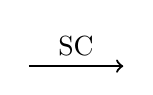
\begin{tikzpicture}[baseline={(current bounding box.center)}, scale=0.2]
            % Arrow from first grid to second grid
            \draw[->, thick] (0, 0) -- (6, 0)
            node[midway, above] {SC};
        \end{tikzpicture}
        \hspace{10pt} % Decrease space here

        \renewcommand{\arraystretch}{1.5} % Adjust the row height
        \setlength{\tabcolsep}{0pt} % Remove extra padding between columns
        \begin{array}{|p{0.5cm}|p{0.5cm}|p{0.5cm}|p{0.5cm}|} % Fixed column width
            % \begin{array}{|p{0.2cm}|p{0.2cm}|p{0.2cm}|p{0.2cm}|}
            \hline
            ? & ? & ? & ? \\ \hline
            ? & ? & ? & ? \\ \hline
            ? & ? & ? & ? \\ \hline
            ? & ? & ? & ? \\ \hline
        \end{array}
        \hspace{20pt} % Decrease space here
        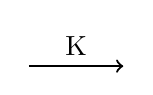
\begin{tikzpicture}[baseline={(current bounding box.center)}, scale=0.2]
            % Arrow from second grid to third grid
            \draw[->, thick] (0, 0) -- (6, 0)
            node[midway, above] {K};
        \end{tikzpicture}
        \)
    }
\end{center}